\section{Additional Experimental Details}
\label{app:details}

This supplement preserves the epistemic role of the complementary negative evidence and provides compact details for the secondary CKA analysis and the post-closure construct-sensitivity audit. It is not a chronological archive of every project experiment. All claims remain bounded to the registered models, carrier, task panel, splits, and conditions.

\subsection{Complementary-split recovery}
EXP-023 was a registered version-controlled replication of the restricted-recovery question under a complementary split. Split A shows recovery under the registered endpoint, whereas Split B does not. The registered cross-split outcome is \texttt{NO\_REPLICATION}.

This result is evidence of split heterogeneity. It does not show that recovery is absent in every setting, and it is not relabeled as a partial replication by pooling the two splits. Recalibration is an operational diagnostic here, not a mechanism claim.

\begin{figure}[h]
\centering
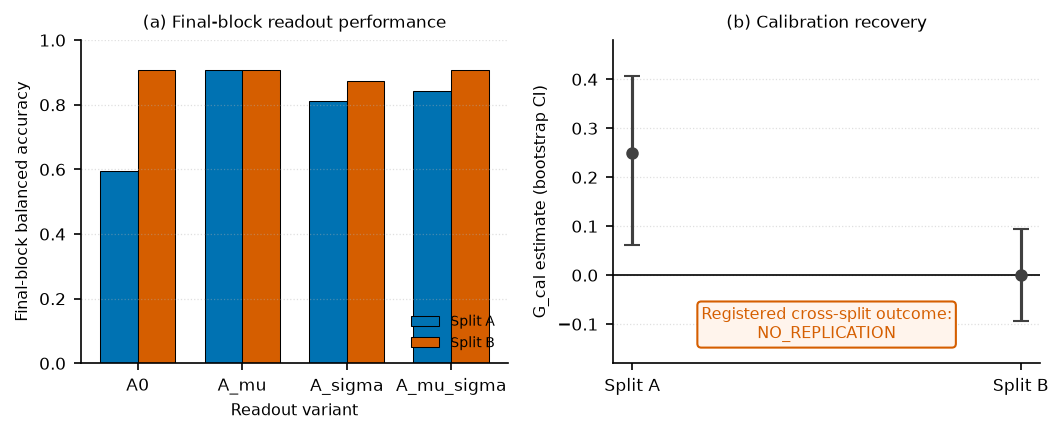
\includegraphics[width=.82\linewidth]{../appendix/figures/fig04.png}
\caption{EXP-023 complementary-split result. Split A supports the registered recovery endpoint and Split B does not; the registered outcome is \texttt{NO\_REPLICATION}. The figure reports the existing validated asset and does not imply uniform recovery or its absence everywhere.}
\end{figure}

\subsection{Registered degradation-based predictor}
EXP-024 tested the registered diagnostic predictor using all 10 registered conditions. The diagnostic is $S_{\mathrm{diag}}(c)$ and the outcome is $G_{\mathrm{eval}}(c)$. The registered association was Spearman $\rho=0.28401877872187725$, with exact one-sided $p=0.2115079365079365$; the registered outcome was \texttt{NOT\_SUPPORTED}.

No post-hoc subset, positivity inference, trend-significance claim, or power-adjusted rescue is introduced. The result limits the interpretation of a single degradation-based scalar predictor; it does not show that no relationship exists under any other measurement or design.

\begin{figure}[h]
\centering
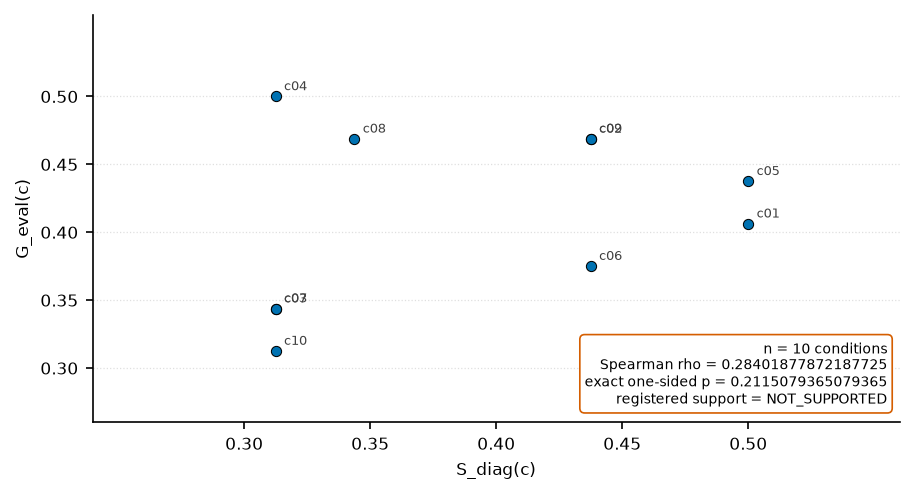
\includegraphics[width=.82\linewidth]{../appendix/figures/fig05.png}
\caption{EXP-024 registered predictor test across all 10 conditions. The plotted diagnostic is $S_{\mathrm{diag}}(c)$ and the outcome is $G_{\mathrm{eval}}(c)$; the exact one-sided test gives $\rho=0.28401877872187725$ and $p=0.2115079365079365$, with registered outcome \texttt{NOT\_SUPPORTED}.}
\end{figure}

\subsection{Secondary CKA comparison}
CKA uses the EVAL split, 640 samples per model, the post-block residual carrier before final normalization, and centered linear CKA. The table reports model-wise off-diagonal Spearman associations; models are not pooled.

\begin{table}[h]
\caption{Secondary CKA associations.}
\centering
\begin{tabular}{lrrr}
\toprule
Model & CKA vs. $C0$ & CKA vs. $D$ & CKA vs. $R$\\
\midrule
Qwen & 0.8372 & -0.8373 & -0.6738\\
OLMo & 0.7589 & -0.8082 & -0.3729\\
Llama & 0.7706 & -0.7634 & -0.5189\\
\bottomrule
\end{tabular}
\end{table}

These are descriptive associations and comparisons with completed operational measurements. CKA is symmetric by construction and does not establish causality, mechanism, information flow, geometry, or equivalence.

\subsection{Post-closure construct-sensitivity audit}
This audit is \texttt{POST\_CLOSURE\_DESCRIPTIVE\_SENSITIVITY}, not confirmatory evidence. Module A exposes the already registered SDI components. Module B0 exposes the already registered LOW-D auxiliaries. Module B1 reports the new, descriptive EVAL headroom summary using the exact DIAGNOSTIC-defined LOW-D mask. The mask is eligible source rows, off-diagonal pairs, and $D^{\mathrm{DIAG}}(i,j)\leq0$; DIAG denotes the DIAGNOSTIC split, not a matrix diagonal, and the mask is not selected from EVAL.

\begin{table}[h]
\caption{Exact canonical three-model profile values and displayed bootstrap bounds.}
\centering
\scriptsize
\resizebox{\linewidth}{!}{%
\begin{tabular}{lrrrrrrrrrrrrrrrr}
\toprule
Model & Distance association & Distance 5\% & Distance 95\% & Distance status & SDI & SDI 5\% & SDI 95\% & SDI class & LOW-D mean & LOW-D 5\% & LOW-D 95\% & Selected pairs & Positive-R fraction & Evaluability & LOW-D support\\
\midrule
Qwen3-1.7B & 0.7049462572 & 0.6851830381 & 0.7080622075 & POSITIVE\_SUPPORTED & -0.1735535241 & -0.1886852743 & -0.1582748746 & TARGET\_DOMINANT & 0.0001392327 & -0.0000993316 & 0.0003610766 & 202 & 0.0742574257 & EVALUABLE & NOT\_SUPPORTED\\
OLMo-2-1B-Instruct & 0.7519250368 & 0.7438987161 & 0.7582397801 & POSITIVE\_SUPPORTED & 0.5249651786 & 0.4910149189 & 0.5584696075 & SOURCE\_DOMINANT & 0.0478571431 & 0.0440289896 & 0.0515186089 & 35 & 0.8285714286 & EVALUABLE & SUPPORTED\\
Meta-Llama-3.2-1B-Instruct & 0.6077483253 & 0.5949008758 & 0.6154160155 & POSITIVE\_SUPPORTED & -0.4142642299 & -0.4342173412 & -0.3923962803 & TARGET\_DOMINANT & 0.0014030612 & 0.0007325690 & 0.0021867916 & 49 & 0.3265306122 & EVALUABLE & SUPPORTED\\
\bottomrule
\end{tabular}}
\end{table}

The corresponding registered support labels are positive-supported distance association for all three models; Qwen LOW-D is \texttt{NOT\_SUPPORTED}, while OLMo and Llama LOW-D are \texttt{SUPPORTED}. Qwen, OLMo, and Llama positive-$R$ fractions are 0.0742574257, 0.8285714286, and 0.3265306122, respectively. The selected-pair counts and interval convention are registered quantities, not majority-vote or normalized-capacity measures.

\subsection{Registered conditions and split boundary}
The ten conditions vary lexical realization, syntactic structure, compression/elaboration, relation explicitness, formal/informal register, a neutral distractor prefix, and anaphoric reference while retaining the registered semantic-class identity. The source-family split prevents related surface conditions from crossing FIT, DIAGNOSTIC, and EVAL. The source readout is fit on FIT only; the restricted calibration may use target-depth FIT representations for its registered featurewise statistics. EVAL labels and outcomes cannot change coefficients, calibration, or pair membership.

\subsection{Artifact and reproducibility index}
The primary result authorities are the version-controlled EXP-022A, EXP-023, EXP-024, EXP-025, EXP-026, and EXP-027 result artifacts, together with the scientific asset register and relevant version-controlled protocol artifacts. The main manuscript records the carrier, source/target indexing convention, classifier and calibration settings, split structure, bootstrap unit, and registered thresholds. Exact hashes and artifact paths are available through the anonymous artifact package.

The full condition-pooled C0, D, and R matrices are available through the machine-readable supplementary artifact and are summarized visually only for D in the main manuscript. The EXP-025 route remains part of the main-text evidence chain: the tested OLMo panel records cross-model heterogeneity in the degradation/recovery profile while its separate degradation-based predictor remains unsupported. No new EXP-025 visualization is introduced in this supplement.

\subsection{Claim boundary}
These materials support statements about measured direct fixed-readout compatibility, degradation, restricted recalibratability under the registered operator, model-dependent profiles, and descriptive association with a secondary symmetric similarity measure. They do not support causal, mechanistic, information-flow, geometric, universal, or deployment claims.
